\documentclass[12pt,a4paper,oneside, titlepage]{article}
\usepackage[left=2cm,right=2cm,top=2cm,bottom=2cm]{geometry}
\usepackage[pdftex]{graphicx}
\usepackage[final]{pdfpages}
%\usepackage[frenchb]{babel}
\usepackage[utf8]{inputenc}
\usepackage{cite}
\usepackage{hyperref}
\begin{document}
\newcommand{\spherotitle}[2]{
\begin{titlepage}
\begin{center}

\includegraphics[scale=1.50]{../UMONS.jpg}\\[0.4cm]

\includegraphics[scale=0.30]{../FS_Logo.jpg}\\[3cm]
{\Large Un réseau de neurones pour la}\\

\includegraphics[scale=0.30]{../sphero.jpg}\\
\rule{8cm}{0.5mm}\\[0.5cm]
{\huge \bfseries #1}\\[0.2cm]
\rule{8cm}{0.5mm}\\[7cm]
% Author and supervisor. Come from http://www.jujens.eu/posts/2013/Oct/20/latex-page-garde/
    \begin{minipage}{0.4\textwidth}
      \begin{flushleft} \large
        Jason \textsc{Bury}\\
        130538\\
        Master 1 en\\Science-informatique\\
      \end{flushleft}
    \end{minipage}
    \begin{minipage}{0.4\textwidth}
      \begin{flushright} \large
        \emph{Codirecteurs :}~~\\M. Pierre \textsc{Hauweele}\\M. Hadrien \textsc{Mélot}\\
        \emph{Rapporteur : }~~\\M. Tom \textsc{Mens}
      \end{flushright}
    \end{minipage}
   \vfill
  {\large #2}
\end{center}
\end{titlepage}
}
\newcommand{\terminologie}{
\begin{figure}
 \begin{center}
 \underline{\hypertarget{terminologie}{Terminologie}}\\
 \begin{tabular}{|l|l|}
  \hline
  Terme & Nom anglais complet\\
  \hline
  ANN & Artificial Neural Network\\
  ELM & Extreme Learning Machine\\
  FNN & Feedforward Neural Networks\\
  MLP & Multilayer Perceptron\\
  RBF & Radial Basis Function\\
  CNN & Convolutional neural Network\\
  RNN & Recurrent Neural Network\\
  SRN & Simple Recurrent Network\\
  ESN & Echo State Network\\
  LSM & Liquid State Machine\\
  SNN & Spiking Neural Network\\
  LSTM & Long Short-Term Memory\\
  BRNN & Bi-directional Recurrent Neural Network\\
  RMLP & Recurrent Multilayer Perceptron\\
  \hline
 \end{tabular}
 \end{center}
 \caption{Terminologie des réseaux de neurones}
 \label{terminologie}
\end{figure}
}

\newcommand{\termi}[1]{\hyperlink{terminologie}{\uppercase{#1}} }
\newcommand{\rbf}{\termi{rbf}}
\newcommand{\mlp}{\termi{mlp}}
\newcommand{\rmlp}{\termi{rmlp}}
\newcommand{\srn}{\termi{srn}}
\newcommand{\ann}{\termi{ann}}
\newcommand{\lsm}{\termi{lsm}}

\newcommand{\rna}{\hyperlink{rna}{RNA} }
\newcommand{\ubf}[1]{\textbf{\underline{#1}}}
\newcommand{\enum}[1]{\og #1 \fg}%{\og\textbf{#1}\fg}
\newcommand{\captionsource}[2]{
  \caption[{#1}]{
    #1
    \\\hspace{\linewidth}
    \textbf{Source:} #2
  }
}

\newcommand{\partiel}[2]{\frac{\partial #1}{\partial #2}}
\newtheorem{definition}{Définition}
\newtheorem{thm}{Théorème}
\spherotitle{Pré-rapport}{Décembre 2016}
\tableofcontents
\newpage
\section{Introduction}
\subsection*{Énoncé}
Ce projet consiste à implémenter un \emph{réseau de neurones artificiels} \hypertarget{rna}{(RNA)} de commander la Sphero.
Il devra effecter n'importe quel trajectoire et aussi des trajectoire à grande vitesse et gèrer les dérapages.
La Sphero sera commandé sur un sol plat sans obstacle.
\subsection*{Avantages d'un réseau de neurones}
\begin{itemize}
 \item \textbf{parallélisme}: L'apprentissage et la génération de vecteur de sortie est massivement parallélisable dans un RNA.\cite{corelet,Haykin}
 \item \textbf{Généralisation}: Répond de manière raisonnable à une entrée non rencontrée durant la phase d'apprentissage.\cite{statistica,Haykin}
 \item \textbf{Approximation non-linéaire}: Les RNA présentés dans ce rapport sont des approximateurs universels de fonctions non-linéaires.\cite{Haykin}
 \item \textbf{Adaptabilité}: Un RNA avec apprentissage on-line s'adapte aux changements dans le système.\cite{Haykin}
 \item \textbf{Boite noire}: Un RNA agit comme une boite noire. L'utilisateur n'a pas besoin de connaitre le fonctionnement du réseaux.
 \item \textbf{Tolérance au bruit}: Le bruitage dans la phase d'apprentissage impacte peu les performances d'un RNA.\cite{Haykin}
\end{itemize}
C'est grâce à ces avantages qu'un réseaux de neurones artificiels peut être intéressant pour commander la Sphero.
En effet, Il est très difficile de générer les commandes de manières analytique fidèle à la réalité à cause des trop nombreux paramètres à gèrer (Centre de gravité changeant, frottement, dérapages, équilibre, défauts,...).
Grâce au fait qu'un RNA agit comme une boite noire et est approximateur universel de fonction, nous pouvons nous passer de la conception d'un simulateur ou d'une tentative de formule analytique pour génerer les commandes.
De plus, si l'apprentissage se fait on-line, le réseau de neurones pourra s'adapter si le coefficient de frottement du sol change ou si il y une modification à la Sphero.
Et enfin, nous aurons invévitablement des bruitages dans les données fournies par les capteurs.

\section{Principaux réseaux de neurones artificiels}
\terminologie
\subsection{Perceptron mutli-couches (MLP)}
\subsubsection*{Neurone}
\begin{figure}
 \centering
 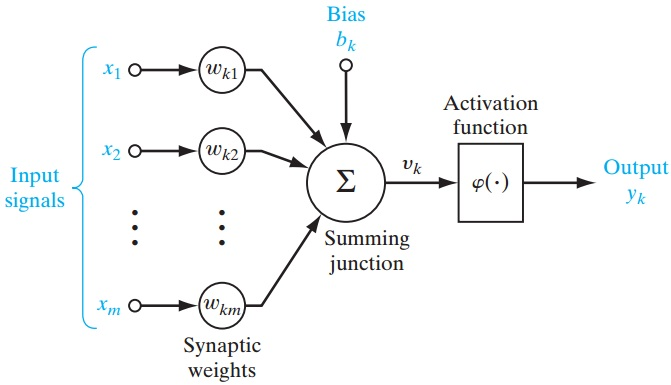
\includegraphics[scale=0.5]{../figures/neurone.jpg}
 \caption{Un neurone artificiel. \textbf{Source}: Haykin\cite{Haykin}}
 \label{neuronemlp}
\end{figure}
\begin{figure}
 \centering
 %insert tableau de statistica here
 \textbf{Tableau STATISTICA}
 \caption{Fonctions principalement utilisés dans un neurone d'un MLP. \textbf{Source}: STATISTICA Réseaux de Neurones Automatisés (SANN)\cite{statistica}}
 \label{mlpfonc}
\end{figure}
Tout d'abord focalisons-nous sur le travail d'un neurone (Figure \ref{neuronemlp}).
Un neurone effectue tout d'abord une somme pondérée $v = b+\sum_{i=0}^{m}x_{i}w_{i}$ de ses entrées.
Chaque terme est mutiplié par un poid $w$. Ce sont les poids qui seront modifiés lors de la phase d'apprentissage.
Ensuite il applique la fonction $\phi(x)$ sur la somme pondérée.
Le domaine de $y$ est généralement $[0,1]$ ou $[-1,1]$.\cite{Haykin}
La fonction $\phi(x)$ utilisé dépend du problème qu'on veut résoudre (Figure \ref{mlpfonc}).
\subsubsection*{Structure}
\begin{figure}
 \centering
 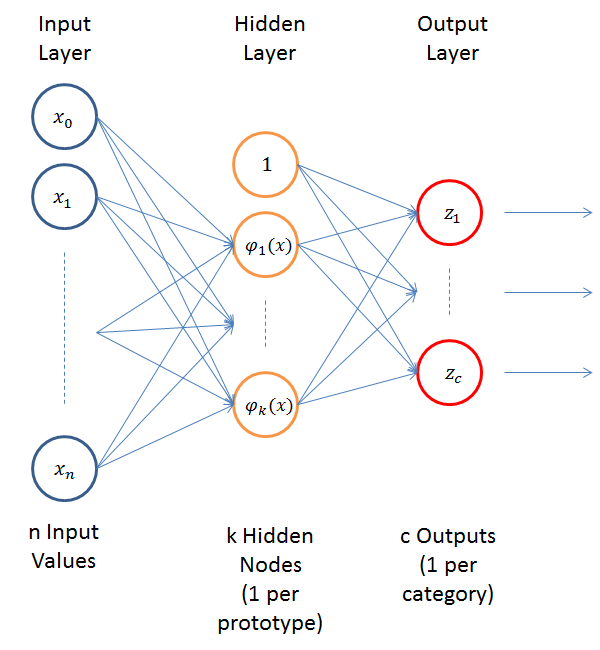
\includegraphics[scale=0.5]{../figures/nnstruct.png}
 \caption{Structure MLP à une couche cachée. \textbf{Source}: McCormick\cite{RBFtuto}}
 \label{structuremlp}
\end{figure}
Un \mlp est composé de plusieurs couches (Figure \ref{structuremlp}):\\
couche d'entrée $\rightarrow$ couches cachées $\rightarrow$ couche de sortie.
Un neurone envoie sa sortie vers tous les neurones de la couche suivante.
Chaque neurones de la couche d'entrée correspond à une dimension du vecteur d'entrée et renvoie juste la valeur de l'entrée dans cette dimension.
Chaque neurones de sortie correspond à une dimension du vecteur de sortie. %TODO quelle fonction ?
Chaque neurones cachés correspond à un neurones de la Figure \ref{neuronemlp}.
\subsubsection*{Applications}
À une couche cachée, un \mlp peut déja servir dans la prédiction de profil.\cite{statistica}\\
Les \mlp sont aussi utilisés en commande de robot par caméra.\cite{Pomerleau}

\subsection{Base radiale (RBF)}
\subsubsection*{Neurone}
Un neurone d'un \rbf n'effectue pas de somme pondérée de ses entrées. Il applique directement sa fonction \[\phi(x) = e^{-\beta||x-\mu||^2}\]
Où $x$ est l'entrée, $\mu$ le prototype, $\beta$ le coefficient qui règle la largeur de la courbe en cloche. $x$ et $\mu$ sont des vecteurs.
\begin{figure}
 \centering
 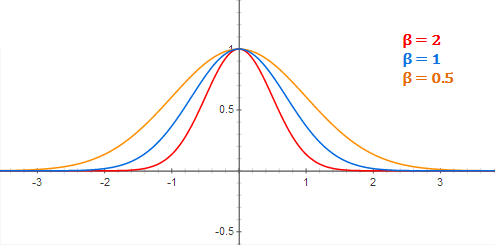
\includegraphics[scale=0.7]{../figures/RBFactivation.png}
 \caption{Activation d'un neurone RBF avec différentes valeurs pour $\beta$}
 \label{rbfactivation}
\end{figure}
La Figure \ref{rbfactivation} représente la sortie d'un neurone \rbf où $\mu$ et $x$ sont de dimension 1 et $\mu = 0$.\\
Pour résumer, un neurone \rbf renvoie une valeur indiquant la simularité entre l'entrée et son prototype.
\subsubsection*{Structure}
\begin{figure}
 \centering
 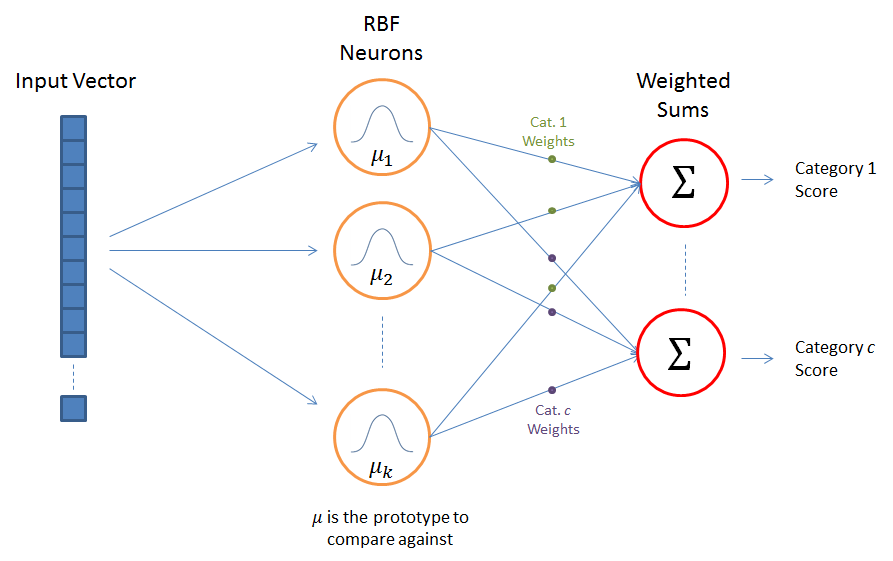
\includegraphics[scale=0.5]{../figures/RBFstruct.png}
 \caption{Structure RBF. \textbf{Source}: McCormick\cite{RBFtuto}}
 \label{structurerbf}
\end{figure}
La structure d'un \rbf est comme celle du \mlp sauf qu'il n'y a qu'une seule couche cachée (Figure \ref{structurerbf}).
\subsubsection*{Applications}
Un \rbf peut aussi servir dans la prédiction de profil.\cite{statistica}

\subsection{Convolutif (CNN)}
\subsection{Récurrent (RNN)}
\subsubsection*{Structure}
\begin{figure}
 \centering
 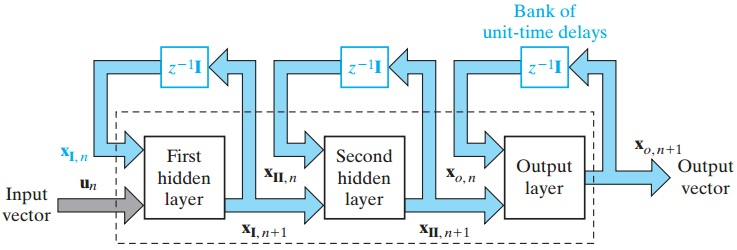
\includegraphics[scale=0.5]{../figures/structurermlp.jpg}
 \caption{Structure RLMP. \textbf{Source}: Haykin. p795\cite{Haykin}}
 \label{structurermlp}
\end{figure}
\begin{figure}
 \centering
 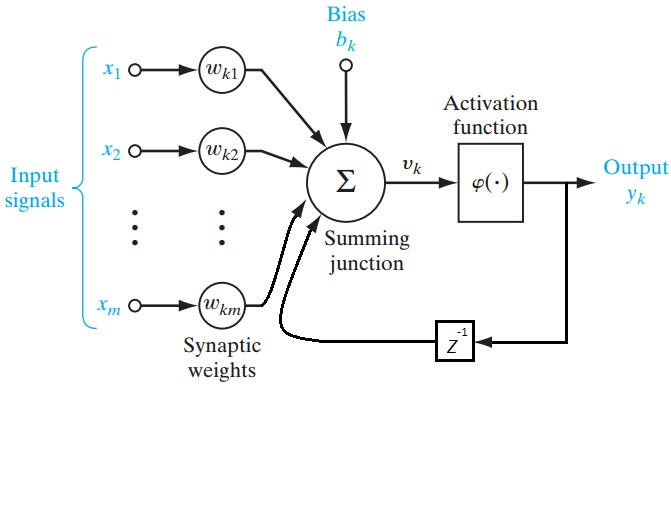
\includegraphics[scale=0.5]{../figures/neuronermlp.jpg}
 \caption{Neurone caché d'un RMLP}
 \label{neuronermlp}
\end{figure}
Un réseau de neurones récurrent est un réseaux présentant des boucles dans sa structure.
Des \enum{retardeurs} notés $Z^{-1}$ sont présents sur certains arcs dans le réseau afin de retarder d'une étape la transmission d'une valeur.
Une étape dans un réseau consiste à recevoir une entrée et en générer une sortie.
Il existe plusieurs réseaux de type récurrent (récurrent simple, machine à états liquide, etc).
La Figure \ref{structurermlp} Présente un réseau de type perceptron multi-couches récurrent (\rmlp).
Il s'agit d'un \mlp dont les neurones de la couches cachée ont un arc qui boucle sur le neurone lui-même avec un $Z^{-1}$ sur cet arc, comme sur la Figure \ref{neuronermlp}.
\subsubsection*{Applications}
Grâce aux \enum{retardeurs} $Z^{-1}$, le réseau peut approximer des fonctions dont la sortie ne dépend pas seulement de l'entrée actuelle mais aussi des entrées précédentes.
Par exemple, le réseau de neurones récurrent simple (\srn), qui est un \rmlp à une seule couche cachée, peu déja effectuer des prédictions de symbole en suivant une séquence.
Les \emph{machines à états liquides} (\lsm), donc les connections se font de manière aléàtoire, sont utilisés pour la reconnaissance automatique de la parole. %TODO citer
Les \emph{long-short term memory} sont utilisés pour la reconnaissance automatique de la parole ou de l'écriture manuscrite. %TODO citer

\subsection{CMAC}
\section{Architectures}
\section{Design du vecteur d'entrée}
\subsection{Données utiles}
Avant de choisir le réseau de neurones à utiliser, il est important d'identifier ce que nous souhaitons obtenir en sortie et les informations que nous pouvons fournir en entrée sans fournir des données inutiles.
Si le vecteur d'entrée est de dimension très grande, alors un réseau \rbf devra avoir un trop grand nombre de neurones cachés\cite{Gauthier}.
Si nous supposons que la sortie produite peut dépendre non seulement de l'input actuel mais aussi des entrées précédentes, alors un réseau récurrent devra être utilisé.

La Sphero peut nous fournir:\cite{SDKofficiels}
\begin{itemize}%TODO les unités
 \item Sa position grâce à un odomètre (cm),
 \item Son vecteur vitesse (mm/s),
 \item Son vecteur d'accélération grâce à un accéleromètre (mG),
 \item Son orientation (-179$\rightarrow$180 degrés),
 \item Son niveau de charge (Label \enum{En charge}, \enum{OK}, \enum{Bas}, \enum{Critique}),
 \item État des LEDs, évènement de collision, voltage de la batterie, nombre de charges, version ...
\end{itemize}

Parmis ces données, nous n'avons pas besoin de l'état des LEDs, version et nombre de charges car ils n'influencent pas la conduite de la Shero.
Dans ce projet, nous ne prenons pas en compte les éventuels collisions.

Le niveau de charge pourrait influencer la conduite.
Il se pourrait que la puissance maximale des moteurs diminuent lorsque la charge est trop faible.
Pour ne pas devoir effectuer un entrainement pour chaque niveau de charge différente, on entrainera la Sphero que pour les cas où le niveau de charge est à \enum{OK} et on supposera donc que la conduite sera effectuée qu'avec ce niveau de charge.

Pour l'accélération, les commandes à appliquer à l'instant $t$ ne dépendent pas de l'accélération à l'instant $t$ juste avant l'application des commandes.
Mais par contre, cette donnée peut être utile pour anticiper la vitesse de la Sphero au moment où elle reçoit les commandes car du à la latence d'envoi de paquet, la vitesse à l'instant $t$ n'est plus la même que celle communiquée.
Si cette donnée impacte peu dans les résultats obtenus, alors nous pourrions décider de nous passer de ce paramètre.
Ajouter cette dimension dans le vecteur d'entrée demandera un plus grand nombre d'exemples pour la phases d'apprentissage car il faut balayer toutes les configurations possibles de vecteur d'entrée.

\subsection{Choix du design}
 %TODO montrer les design repris chez gauthier

La vitesse maximale de la Sphero est de 4,5 miles par heure\cite{product}.
Ce qui fait environ 2 mètres pas seconde.
%Or les temps de récéption de ping après envoi son de 9ms avec quelque pics allants jusqu'à 37ms. TODO meilleurs mesures
Pour de meilleures précisions, on ajoute un vecteur vitesse à atteindre sur le point de destination.
On aligne l'axe des abscisses avec l'axe de l'orientation du moteur afin de reduire le domaine d'entrée et donc le nombre d'exemples à créer pour l'apprentissage.
Le vecteur d'entrée contiendra donc le vecteur vitesse, la position relative à atteindre dans $T$ secondes où $T$ sera la période à laquelle on échantillonera les données des capteurs et le vecteur vitesse à atteindre sur cette position de destination.
Nous avons donc un vecteur d'entrée à 6 dimensions.
Le vecteur de sortie sera la puissance à donner pour les deux moteurs.

\section{Choix du réseau}
Nous n'avons pas besoin d'un réseau de neurones récurrent. Les commandes à appliquer au moment $t$ ne dépendent pas de la vitesse, position et autres données fournies à $t-T$.
Le réseau le mieux adapté pour notre problème est un réseau de neurones à base radial.
En effet, les \rbf sont moins sensibles au bruit que les \mlp \cite{adversarial,Gauthier}.%gauthier p 39,40
%TODO pourquoi
Un inconvénient des \rbf, celui du nombre de neurones cachés qui croît avec la dimension et la taille du vecteur d'entrée, ne pose pas de problème dans notre cas
car le nombre de dimensions est faible
et le domaine d'entrée est assez faible pour chaque dimensions.
\section{Choix de l'API}
Les APIs officiels sont:\cite{SDKofficiels} \textbf{Objective-C}, \textbf{Swift}, \textbf{Android}.\\
Il existe également des APIs créé par la communauté:\cite{gosphero} \textbf{C\#}, \textbf{JavaScript}, \textbf{Ruby}, \textbf{Python}\cite{pythonAPI}, \textbf{Arduino}, \textbf{C++}\cite{cppAPI}.\\
%TODO
\section{Conclusion}
\subsection*{Remerciements}
\noindent Je remercie monsieur Pierre \textsc{Hauweele} de m'avoir proposé un projet qui est exactement dans le domaine que je voulais, de son aide et d'avoir choisi d'être directeur de mon projet.\\

\noindent Je remercie monsieur Hadrien Mélot d'être directeur de mon projet et de l'aide qu'il m'a apporté.\\

\noindent Je remercie monsieur Tom Mens d'être rapporteur de mon projet et de son aide.\\

\bibliographystyle{plain}
\bibliography{../bibli}
\end{document}
